%% Except where otherwise noted, content in this documentation is Copyright (c)
%% 2022, RTE (http://www.rte-france.com) and licensed under a
%% CC-BY-4.0 (https://creativecommons.org/licenses/by/4.0/)
%% license. All rights reserved.

\documentclass[a4paper, 12pt]{report}
% Latex setup
%% Except where otherwise noted, content in this documentation is Copyright (c)
%% 2022, RTE (http://www.rte-france.com) and licensed under a
%% CC-BY-4.0 (https://creativecommons.org/licenses/by/4.0/)
%% license. All rights reserved.

% Latin Modern fam­ily of fonts
\usepackage{lmodern}

\usepackage[english]{babel}

% specify encoding
\usepackage[utf8]{inputenc} % input
\usepackage[T1]{fontenc} % output

% Document structure setup
\usepackage{titlesec} % To change chapter format
\setcounter{tocdepth}{3} % Add subsubsection in Content
\setcounter{secnumdepth}{3} % Add numbering for subsubsection
\setlength{\parindent}{0pt} % No paragraph indentation

% Change title format for chapter
\titleformat{\chapter}{\Huge\bf}{\thechapter}{20pt}{\Huge\bf}

% To add links on page number in Content and hide red rectangle on links
\usepackage[hidelinks, linktoc=all]{hyperref}
\usepackage[nottoc]{tocbibind}  % To add biblio in table of content
\usepackage{textcomp} % For single quote
\usepackage{url} % Allow linebreaks in \url command
\usepackage{listings} % To add code samples

% Default listings parameters
\lstset
{
  aboveskip={1\baselineskip}, % a bit of space above
  backgroundcolor=\color{shadecolor}, % choose the background color
  basicstyle={\ttfamily\footnotesize}, % use font and smaller size \small \footnotesize
  breakatwhitespace=true, % sets if automatic breaks should only happen at whitespace
  breaklines=true, % sets automatic line breaking
  columns=fixed, % nice spacing -> fixed / flexible
  mathescape=false, % escape to latex false
  numbers=left, % where to put the line-numbers
  numberstyle=\tiny\color{gray}, % the style that is used for the line-numbers
  showstringspaces=false, % do not emphasize spaces in strings
  tabsize=4, % number of spaces of a TAB
  texcl=false, % activates or deactivates LaTeX comment lines
  upquote=true % upright quotes
}

% Avoid numbering starting at each chapter for figures
\usepackage{chngcntr}
\counterwithout{figure}{chapter}

\usepackage{tikz} % macro pack­age for cre­at­ing graph­ics
\usepackage{pgfplots} % draws func­tion plots (based on pgf/tikz)
\pgfplotsset{enlarge x limits=false, xlabel={\begin{small}$time$ (s)\end{small}}, height=0.6\textwidth, width=1\textwidth,
yticklabel style={text width={width("$-0.6$")},align=right},
/pgf/number format/precision=4}
\pgfplotstableset{col sep=semicolon}

\usepackage{algorithm} % Add algorithms
\usepackage[noend]{algpseudocode} %  all end ... lines are omitted in algos

\usepackage{amsmath} % Add math­e­mat­i­cal fea­tures
\usepackage{schemabloc} % Add block diagram library (french one)

\usepackage{adjustbox} % Add box for flowchart

\usepackage{booktabs} % for toprule and midrule in tables

\usepackage{tabularx}

\usepackage[nolist]{acronym} % don’t write the list of acronyms.
% Acronyms list
\begin{acronym}
\acro{BDF}{Backward Differentiation Formula}
\acro{BE}{Backward Euler}
\acro{DAE}{Differential Algebraic Equations}
\acro{IDA}{Implicit Differential-Algebraic solver}
\acro{LLNL}{Lawrence Livermore National Lab}
\acro{KINSOL}{Krylov Inexact Newton SOLver}
\acro{NR}{Newton-Raphson}
\acro{PLL}{Phase-Locked Loop}
\acro{SVC}{Static Var Compensator}
\acro{SUNDIALS}{SUite of Nonlinear and DIfferential/ALgebraic equation Solvers}
\end{acronym}

% Syntax highlight
%% Except where otherwise noted, content in this documentation is Copyright (c)
%% 2022, RTE (http://www.rte-france.com) and licensed under a
%% CC-BY-4.0 (https://creativecommons.org/licenses/by/4.0/)
%% license. All rights reserved.

\usepackage{color}

\definecolor{blue}{rgb}{0,0,1}
\definecolor{lightblue}{rgb}{.3,.5,1}
\definecolor{darkblue}{rgb}{0,0,.4}
\definecolor{red}{rgb}{1,0,0}
\definecolor{darkred}{rgb}{.56,0,0}
\definecolor{pink}{rgb}{.933,0,.933}
\definecolor{purple}{rgb}{0.58,0,0.82}
\definecolor{green}{rgb}{0.133,0.545,0.133}
\definecolor{darkgreen}{rgb}{0,.4,0}
\definecolor{gray}{rgb}{.3,.3,.3}
\definecolor{darkgray}{rgb}{.2,.2,.2}
\definecolor{shadecolor}{gray}{0.925}

% **********************************************************************************
% Syntax : Bash (bash)
% **********************************************************************************

\lstdefinelanguage{bash}
{
  keywordstyle=\color{blue},
  morekeywords={
    cd,
    export,
    source},
  numbers=none,
  deletekeywords={jobs}
}

% **********************************************************************************
% Syntax : XML
% **********************************************************************************

\lstdefinelanguage{XML}
{
  morestring=[s][\color{purple}]{"}{"},
  morecomment=[s][\color{green}]{<?}{?>},
  morecomment=[s][\color{green}]{<!--}{-->},
  stringstyle=\color{black},
  identifierstyle=\color{blue},
  keywordstyle=\color{red},
  morekeywords={
    xmlns,
    xsi,
    noNamespaceSchemaLocation,
    type,
    source,
    target,
    version,
    tool,
    transRef,
    roleRef,
    objective,
    eventually}
}

% **********************************************************************************
% Syntax : Modelica (modelica)
% **********************************************************************************
\lstdefinelanguage{Modelica}{
  alsoletter={...},
  morekeywords=[1]{ % types
      Boolean,
      Integer,
      Real},
  keywordstyle=[1]\color{red},
  morekeywords=[2]{ % keywords
    algorithm,
    and,
    annotation,
    assert,
    block,
    class,
    connector,
    constant,
    discrete,
    else,
    elseif,
    elsewhen,
    end,
    equation,
    exit,
    extends,
    external,
    false,
    final,
    flow,
    for,
    function,
    if,
    in,
    inner,
    input,
    import,
    loop,
    model,
    nondiscrete,
    not,
    or,
    outer,
    output,
    package,
    parameter,
    public,
    protected,
    record,
    redeclare,
    replaceable,
    return,
    size,
    terminate,
    then,
    true,
    type,
    when,
    while},
  keywordstyle=[2]\color{darkred},
  morekeywords=[3]{ % functions
    abs,
    acos,
    asin,
    atan,
    atan2,
    Complex,
    connect,
    conj,
    cos,
    cosh,
    cross,
    der,
    edge,
    exp,
    fromPolar,
    imag,
    noEvent,
    pre,
    sign,
    sin,
    sinh,
    sqrt,
    tan,
    tanh},
  keywordstyle=[3]\color{blue},
  morecomment=[l][\color{green}]{//}, % comments
  morecomment=[s][\color{green}]{/*}{*/}, % comments
  morestring=[b][\color{pink}]{'}, % strings
  morestring=[b][\color{pink}]{"}, % strings
}

\usepackage{tikz}
\definecolor{blue}{rgb}{.3,.5,1}
\definecolor{red}{rgb}{1,0,0}
\usetikzlibrary{shapes,arrows}
% Define block styles
\tikzstyle{decision} = [diamond, draw, fill=blue!20, 
    text width=4.5em, text badly centered, node distance=3cm, inner sep=0pt]
\tikzstyle{block} = [rectangle, draw, fill=blue!20, 
    text width=5em, text centered, rounded corners, minimum height=4em]
\tikzstyle{line} = [draw, -latex']
\tikzstyle{cloud} = [draw, ellipse,fill=red!20, node distance=3cm,
    minimum height=2em]
    \usetikzlibrary{calc}


\usepackage{xspace} % Define typography
\usepackage{dirtree}
\newcommand{\Dynawo}[0]{Dyna$\omega$o\xspace}


\begin{document}

\title{Configure \Dynawo-algorithms}
\date\today

\maketitle
\tableofcontents

\chapter[Configure Dynawo-algorithms]{Configure \Dynawo-algorithms}

\section{Overview}

The following section will provide information on:
\begin{itemize}
\item How to create the input files depending on the algorithm of interest;
\item How to configure the input files in order to get the  necessary output files to analyse the obtained results;
\end{itemize}


\subsection[Dynawo-algorithms inputs]{\Dynawo-algorithms inputs}
\subsubsection{CS mode: simulation of a jobs file}

The Compute Simulation (CS) mode is a simple wrapper around a \Dynawo simulation. 
The main difference is that the status of each simulation is given as output in a dedicated file.

The inputs are thus the same as a \Dynawo simulation and are described in the latest \Dynawo documentation.\\

The command line required to launch CS mode is the following:

\begin{lstlisting}[language=bash, breaklines=true, breakatwhitespace=false]
$> ./myEnvDynawoAlgorithms.sh CS --input <PATH TO JOBS FILE> --output <PATH TO RESULT FILE>
\end{lstlisting}

for example:

\begin{lstlisting}[language=bash, breaklines=true, breakatwhitespace=false]
$> ./myEnvDynawoAlgorithms.sh CS --input nrt/data/IEEE14/IEEE14_BlackBoxModels/IEEE14.jobs --output results.xml
\end{lstlisting}

This command will launch all simulations described in the \textit{IEEE14.jobs} file 
and provide as output a file \textit{results.xml} containing a description of the final status for all simulations. 
Please refer to the section \ref{Dynawo_algorithms_Outputs_AggrResults} for more details on the output file.

\subsubsection{SA mode: systematic analysis}

The Systematic Analysis (SA) mode can be used to start from a single base simulation and to observe 
if the network remains stable when some events occur (typically N-k scenarios).\\

\begin{center}
\begin{figure}[H]
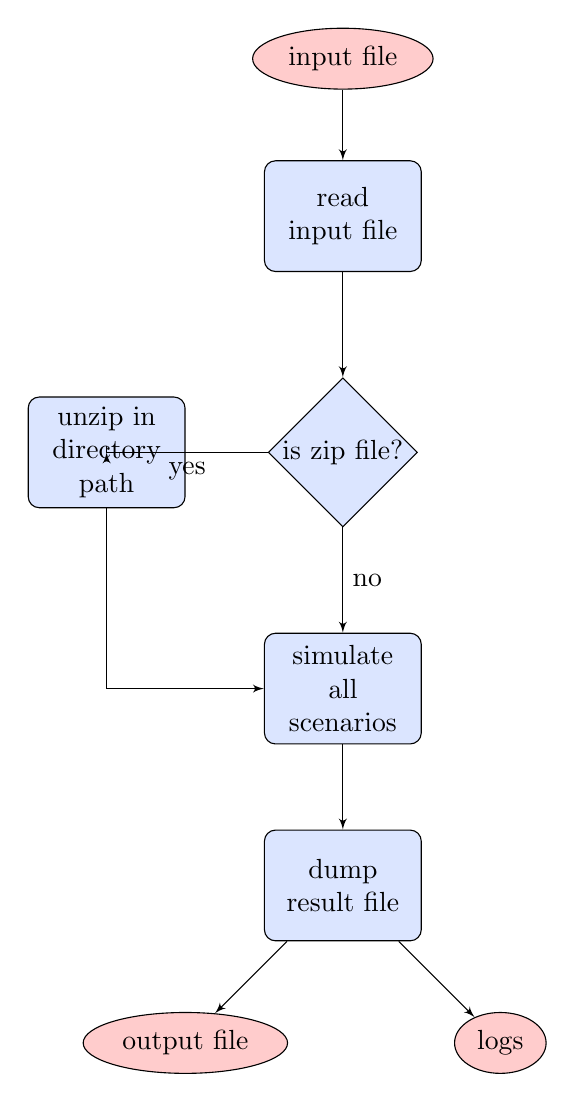
\begin{tikzpicture}[node distance = 2cm, auto]
    % Place nodes
    \node [cloud] (input) {input file};
    \node [block, below of=input] (init) {read input file};
    \node [decision, below of=init] (inputD) {is zip file?};
    \node [block, left of=inputD, node distance=3cm] (unzip) {unzip in directory path};
    \node [block, below of=inputD, node distance=3cm] (Simulate) {simulate all scenarios};
    \node [block, below of=Simulate, node distance=2.5cm] (res) {dump result file};
    \node [cloud, below of=res,left of=res, node distance=2cm] (output) {output file};
    \node [cloud, below of=res,right of=res, node distance=2cm] (logs) {logs};
    % Draw edges
    \path [line] (input) -- (init);
    \path [line] (init) -- (inputD);
    \path [line] (inputD) -| node [near start] {yes} (unzip);
    \path [line] (inputD) -- node {no}(Simulate);
    \path [line] (unzip) |- (Simulate);
    \path [line] (Simulate) -- (res);
    \path [line] (res) -- (output);
    \path [line] (res) -- (logs);
\end{tikzpicture}
\caption{Systematic analysis flow}
\end{figure}
\end{center}

The inputs is a xml multiple jobs file.

\lstinputlisting[language=XML, morekeywords={id},title=multiple jobs file example]{../resources/syntaxExample/SASyntaxExample.xml}

In this example, the base situation is described in \textbf{IEEE14.jobs} file. The format used is the same as a \Dynawo simulation.

Three scenarios will be applied to this base situation: `DisconnectLine', 'Fault` and DisconnectGroup'. 
Each event is described in an additional \textbf{dyd} file that will be added to the base situation. 
The 'Base' scenario has no associated \textbf{dyd} file and will thus simulate to the base situation.

Below is an example of a \textbf{dyd} file for an event:

\lstinputlisting[language=XML, morekeywords={id},title=event dyd file example]{../resources/syntaxExample/event.dyd}

This \textbf{dyd} is added to the one given in \textbf{IEEE14.jobs} and adds a disconnection event to the line '\_BUS\_\_\_\_1-BUS\_\_\_\_5-1'.\\

The command line required to launch SA mode is the following:

\begin{lstlisting}[language=bash, breaklines=true, breakatwhitespace=false]
$> ./myEnvDynawoAlgorithms.sh SA --directory <PATH TO WORKING DIRECTORY> --input <NAME OF INPUT FILE> --output <NAME OF OUTPUT FILE> --nbThreads <NUMBER OF THREADS>
\end{lstlisting}

The default number of thread is 1. The input can be explicit files or zipped ones. For example:

\begin{lstlisting}[language=bash, breaklines=true, breakatwhitespace=false]
$> ./myEnvDynawoAlgorithms.sh SA --directory nrt/data/IEEE14/SA --input fic_MULTIPLE.xml --output results.xml --nbThreads 2
\end{lstlisting}

This command will launch the systematic analysis described in the file \textit{nrt/data/IEEE14/SA/fic\_MULTIPLE.xml} in multi-threading 
and provide as outputs a file named \textit{results.xml} containing the status of each simulated event, 
in addition to the timelines and constraint files of the \Dynawo event simulations.\\

\begin{lstlisting}[language=bash, breaklines=true, breakatwhitespace=false]
$> ./myEnvDynawoAlgorithms.sh SA --directory nrt/data/IEEE14/SA --input inputs.zip --output outputs.zip
\end{lstlisting}

This command will unzip the files contained in \textit{inputs.zip}, launch a SA assuming the input file name is \textit{fic\_MULTIPLE.xml}
and provide as outputs a zipped file named \textit{outputs.zip} containing the status of each simulated event, 
the timelines and constraint files of the \Dynawo event simulations.\\

Please refer to the section \ref{Dynawo_algorithms_Outputs_AggrResults} for more details on the output file.


\subsubsection{MC mode: margin calculation}

The Margin Calculation (MC) mode can be used to start from a single base simulation, to apply a load variation and to observe 
if the network remains stable when some events occur (typically N-k scenarios).\\
The algorithm is as follows: we first simulate the maximum load variation (100\%), and the use the results as the starting point for each event simulation.
If one of those simulation fails, a dichotomy is applied to find out the maximum load variation for which all events (global margin) or each event (local margin) pass.\\

\begin{center}
\begin{figure}[H]
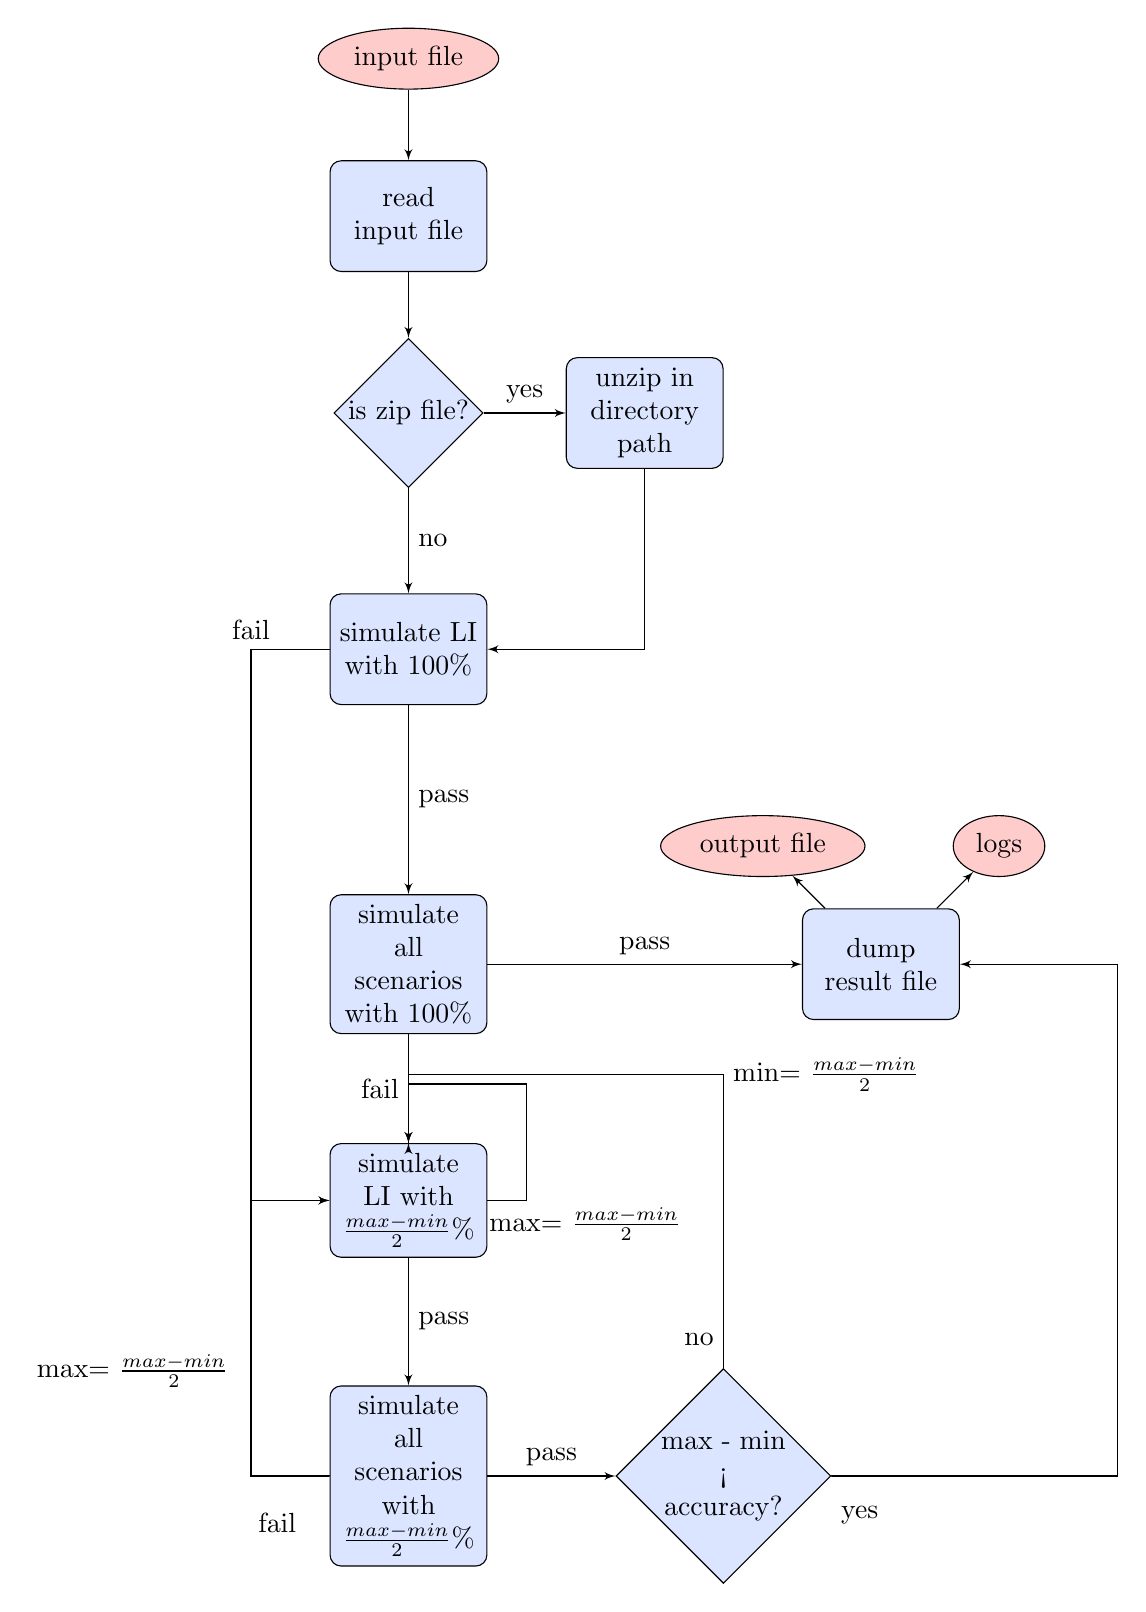
\begin{tikzpicture}[node distance = 2cm, auto]
    % Place nodes
    \node [cloud] (input) {input file};
    \node [block, below of=input, node distance=2cm] (init) {read input file};
    \node [decision, below of=init, node distance=2.5cm] (inputD) {is zip file?};
    \node [block, right of=inputD, node distance=3cm] (unzip) {unzip in directory path};
    \node [block, below of=inputD, node distance=3cm] (SimulateBase100) {simulate LI with 100\%};
    \node [block, below of=SimulateBase100, node distance=4cm] (SimulateAll100) {simulate all scenarios with 100\%};
    \node [block, below of=SimulateAll100, node distance=3cm] (SimulateBaseVar) {simulate LI with $\frac{max-min}{2}$\%};
    \node [block, below of=SimulateBaseVar, node distance=3.5cm] (SimulateAllVar) {simulate all scenarios with $\frac{max-min}{2}$\%};
    \node [decision, right of=SimulateAllVar, node distance=4cm] (OK) {max - min < accuracy?};
    \node [block, right of=SimulateAll100, node distance=6cm] (res) {dump result file};
    \node [cloud, above of=res,left of=res, node distance=1.5cm] (output) {output file};
    \node [cloud, above of=res,right of=res, node distance=1.5cm] (logs) {logs};
    % Draw edges
    \path [line] (input) -- (init);
    \path [line] (init) -- (inputD);
    \path [line] (inputD) -- node {yes} (unzip);
    \path [line] (inputD) -- node {no}(SimulateBase100);
    \path [line] (unzip) |- (SimulateBase100);
    \path [line] (SimulateBase100.west) -| node[above] {fail} (-2,-14.5) |- (SimulateBaseVar.west);
    \path [line] (SimulateBase100) -- node [midway, right] {pass}(SimulateAll100);
    \path [line] (SimulateAll100)  --  node [midway, above] {pass} (res);
    \path [line] (SimulateAll100) -- node [left] {fail} (SimulateBaseVar);
    \path [line] (SimulateBaseVar) -- node {pass} (SimulateAllVar);
    \path [line] (SimulateBaseVar.east) -| node [midway, right, xshift=-0.6cm, yshift=-0.3cm] {max= $\frac{max-min}{2}$} ($(SimulateBaseVar.north east) + (0.5,0.75)$) -|  (SimulateBaseVar);
    \path [line] (SimulateAllVar) -- node {pass} (OK);
    \path [line] (SimulateAllVar.west) |- node [below, left, xshift=-0.3cm, yshift=-0.6cm] {fail} node [above, xshift=-2.5cm, yshift=1cm] {max= $\frac{max-min}{2}$} (-2, -18) |- (SimulateBaseVar.west);
    \path [line] (OK.east) |- node [right,  yshift=-0.5cm] {yes} (9, -18) |- (res.east);
    \path [line] (OK.north) |- node [near start, yshift=-1.5cm] {no}   node [right] {min= $\frac{max-min}{2}$} (0,-12.9) |-(SimulateBaseVar.north);
    \path [line] (res) -- (output);
    \path [line] (res) -- (logs);
\end{tikzpicture}
\caption{Margin calculation flow}
\end{figure}
\end{center}

The inputs is a xml multiple jobs file.

\lstinputlisting[language=XML, morekeywords={id},title=multiple jobs file example]{../resources/syntaxExample/MCSyntaxExample.xml}

In this example, the base initial situation is described in \textbf{IEEE14.jobs} file. The format used is the same as a \Dynawo simulation.
\textbf{This base situation needs to contain the configuration of the maximum load variation that will be applied.}
A load variation can be defined by connecting a \textbf{Variation area} model to the target loads in the \textbf{.dyd} file. 
Please refer to section \ref{Dynawo_Algorithms_Inputs_Load_Variation} for more details.

The initial situation for the events is described in \textbf{IEEE14\_tFin.jobs}. Having two different jobs file allows to modify the dynamic models of nodes if required. 
\textbf{The starting time defined in this .jobs file should be the end time of the load variation jobs file.}
This situation should not contain any load variation model. 

Two scenarios will be applied: `DisconnectLine' and DisconnectGroup'. 
Each event is described in an additional \textbf{dyd} file that will be added to the base situation. 

The margin computed will be the global one with an accuracy of 2\%, meaning that the maximum difference between the result obtained and the exact margin will be 2\%.

The command line required to launch MC mode is the following:

\begin{lstlisting}[language=bash, breaklines=true, breakatwhitespace=false]
$> ./myEnvDynawoAlgorithms.sh MC --directory <PATH TO WORKING DIRECTORY> --input <NAME OF INPUT FILE> --output <NAME OF OUTPUT FILE> --nbThreads <NUMBER OF THREADS>
\end{lstlisting}

The default number of thread is 1. The input can be explicit files or zipped ones. For example:

\begin{lstlisting}[language=bash, breaklines=true, breakatwhitespace=false]
$> ./myEnvDynawoAlgorithms.sh MC --directory nrt/data/IEEE14/MC --input fic_MULTIPLE.xml --output results.xml --nbThreads 2
\end{lstlisting}

This command will launch the margin calculation described in the file \textit{nrt/data/IEEE14/MC/fic\_MULTIPLE.xml} in multi-threading 
and provide as outputs a file named \textit{results.xml} containing the status of all simulations that were run, 
in addition to the timelines and constraint files.\\

\begin{lstlisting}[language=bash, breaklines=true, breakatwhitespace=false]
$> ./myEnvDynawoAlgorithms.sh MC --directory nrt/data/IEEE14/MC --input inputs.zip --output outputs.zip
\end{lstlisting}

This command will unzip the files contained in \textit{inputs.zip}, launch a MC assuming the input file name is \textit{fic\_MULTIPLE.xml}
and provide as outputs a zipped file named \textit{outputs.zip} containing the status of all simulations that were run, 
in addition to the timelines and constraint files.\\

Please refer to the section \ref{Dynawo_algorithms_Outputs_AggrResults} for more details on the output file.

\subsubsection{Load increase mode: simulation of load increase}

This mode is an utility mode to reproduce a simulation of the MC mode at a specific variation.
It uses the same files as the MC mode, except that only a single load variation is simulated.
The command line required to launch the load increase mode is the following:

\begin{lstlisting}[language=bash, breaklines=true, breakatwhitespace=false]
$> ./myEnvDynawoAlgorithms.sh MC --directory <PATH TO WORKING DIRECTORY> --input <NAME OF INPUT FILE> --output <NAME OF OUTPUT FILE> --variation <VALUE BETWEEN 0 AND 100>
\end{lstlisting}

This command will simulate the load variation described in the input file at the level given in the \textit{variation} option.

\subsection[Dynawo-algorithms outputs]{\Dynawo-algorithms outputs}
\label{Dynawo_algorithms_Outputs_AggrResults}

\Dynawo-algorithms results are provided in an 'Aggregated Results' file. This file provides one entry for each simulation and provides the corresponding status.
Possible status of a simulation are the following:
\begin{itemize}
  \item \textbf{CONVERGENCE}: The simulation passed;
  \item \textbf{DIVERGENCE}: The simulation failed with a divergence in the solver;
  \item \textbf{CRITERIA\_NON\_RESPECTED}: The simulation failed with at least one failing criterion;
  \item \textbf{EXECUTION\_PROBLEM}: The simulation failed with another error;
\end{itemize}

An example of 'Aggregated Results' file is given below:

\lstinputlisting[language=XML, morekeywords={id},title=aggregated results file example]{../resources/syntaxExample/SAResults.xml}

In this example, three cases were simulated :
\begin{itemize}
  \item 'DisconnectLine' and 'DisconnectGroup' simulations were successful;
  \item 'Fault' simulation failed with the 'protection' criterion.
\end{itemize}
The global status of the result file is then the worst status of all simulations (CRITERIA\_NON\_RESPECTED in this case).

\subsubsection{CS mode}

the output files of the CS mode are the same as a \Dynawo simulation (outputs described in the \textbf{.jobs}), in addition to an aggregated 
results file with one scenario entry for each job in the input jobs file.


\subsubsection{SA mode}

the output files of the SA mode are the timelines and constraint files for all simulations (if they were requested in the base \textbf{.jobs} file), in addition to an aggregated 
results file with one result per scenario.

\subsubsection{MC mode}

the output files of the SA mode are the timelines and constraint files for all simulations (if they were requested in the base \textbf{.jobs} files), in addition to an aggregated 
results file with one result per load increase and one result per scenario for each variation that were simulated.

\lstinputlisting[language=XML, morekeywords={id},title=MC results file example]{../resources/syntaxExample/MCResults.xml}


\subsubsection{Load variation mode}

the output files of the Load variation mode are the same as a \Dynawo simulation (outputs described in the \textbf{.jobs}), in addition to an aggregated 
results file containing the status of the simulation.

\section[Dynawo input files modification]{\Dynawo-algorithms input files modification}

This section aims at giving more details on input files in order to help the user parametrize its inputs easily and autonomously.

\subsection{MC mode: margin calculation}
\subsubsection{Load variation configuration}
\label{Dynawo_Algorithms_Inputs_Load_Variation}
The load increase is based on the dynamic model \textbf{VariationArea}. Each \textbf{VariationArea} model is connected to the 
\textbf{deltaPc} and \textbf{deltaQc} variables of a subset of loads. 

Please note that \Dynawo support the load increase only on 
loads with no dynamic model defined in the dyd (default model) and with the \textbf{<LOAD NAME>\_isControllable} parameter set to true in the network parameters. 

The \textbf{VariationArea} model increases 
or decreases the active and reactive target powers of the loads linearly in time.

For example, the active power $P$ of a load is computed as shown below. Similar equations are used for reactive power.

$\Delta P$, $startTime$ et $stopTime$ are parameters of the \textbf{VariationArea} model and $P_0$ is the initial power of the load.

\begin{center}
$\Delta P_c(time) = \left\{
    \begin{array}{ll}
        0 & \mbox{si } time<startTime \\
        \frac{\Delta P*(time-startTime)}{stopTime-startTime} & \mbox{si } time \geq startTime \\
        \Delta P & \mbox{si } time \geq stopTime
    \end{array}
\right. $\\
$P(time) = P_0*(1+\Delta P_c(time)) $
\end{center}

When a load increase simulation is launched with a variation $var$ (in \%) during a margin calculation, 
the parameters $\Delta P$, $\Delta Q$, $startTime$ and $stopTime$ of the \textbf{VariationArea} models are adapted so that the final 
active (or reactive) power increase is the following:

\begin{center}
$P = P_0*(1+\frac{\Delta P_c*var}{100}) $
\end{center}

The maximum active (or reactive) power increase is thus:
\begin{center}
$P_{max} = P_0*(1+\Delta P) $\\
\end{center}

\textbf{Warning: to reproduce manually a result, the user will need to adapt not only $\Delta P$ et $\Delta Q$ of the variation model, but also the $stopTime$ 
to reach the proper variation level}

Below is given the example of the active power evolution for one load for $P_0 = 0.94$, $startTime = 10s$, $stopTime=70s$, $\Delta P = 10$ 
and for the variation levels  $var=0$\%, $var=50$\% and $var=75$\%.

\begin{center}
\begin{figure}[H]
  \begin{tikzpicture}
    \begin{axis}[height = 4in]
        \addplot[color=purple!50]
        table[x=time, y=_LOAD___3_EC_P]
        {../resources/syntaxExample/curves-0.csv};
        \addplot[color=blue!50]
        table[x=time, y=_LOAD___3_EC_P]
        {../resources/syntaxExample/curves-75.csv};
        \addplot[color=red!50]
        table[x=time, y=_LOAD___3_EC_P]
        {../resources/syntaxExample/curves-50.csv};
    \end{axis}
    \end{tikzpicture}
\caption{value of $P$ for a variation of 0\%, 50\% and 75\%}
\end{figure}
\end{center}


\end{document}
